\label{cha:design_of_data_and_functionality}

\subsection{Excercise CarRentalEntities}
\label{sec:exercise_car_rental_entities}
\subsubsection*{Description of the Initial Entity Diagram}
The entity diagram consists of the following entities:
\begin{itemize}
    \item Customer entity
    \item Rental entity
    \item Car entity
    \item Date value object
\end{itemize}
A customer has zero ore more rentals.
Therefore each rental belongs to at exactly one customer.
Each rental has a date value object and belongs to exactly one car.

\subsubsection*{Adding the Attributes}
The extended entity diagram is shown in \autoref{fig:extendedEntityDiagram}.
The following attributes are added to the entities:
\begin{itemize}
    \item Customer entity
    \begin{itemize}
        \item id: contains the customer id and identifies the customer
        \item name: contains the name of the customer
        \item creditCard: true if the customer has a valid credit card, false otherwise
        \item rentals: list of rental objects that belong to the customer. The list can be empty if no cars are rented.
    \end{itemize}
    \item Rental entity
    \begin{itemize}
        \item id: contains the rental id and identifies the rental
        \item date: link to the date value object that contains the start and end date of the rental
        \item car: link to the car object that is rented. Can be null if no car is assigned to the rental
    \end{itemize}
    \item Car entity
    \begin{itemize}
        \item id: contains the car id and identifies the car
        \item type: contains the type of the car
        \item rented: true if the car is rented, false otherwise
        \item price: contains the price of the car per day
    \end{itemize}
    \item Date value object
    \begin{itemize}
        \item startDate: contains the start date of the rental
        \item endDate: contains the end date of the rental
    \end{itemize}
\end{itemize}

\begin{figure}[h]
    \centering
    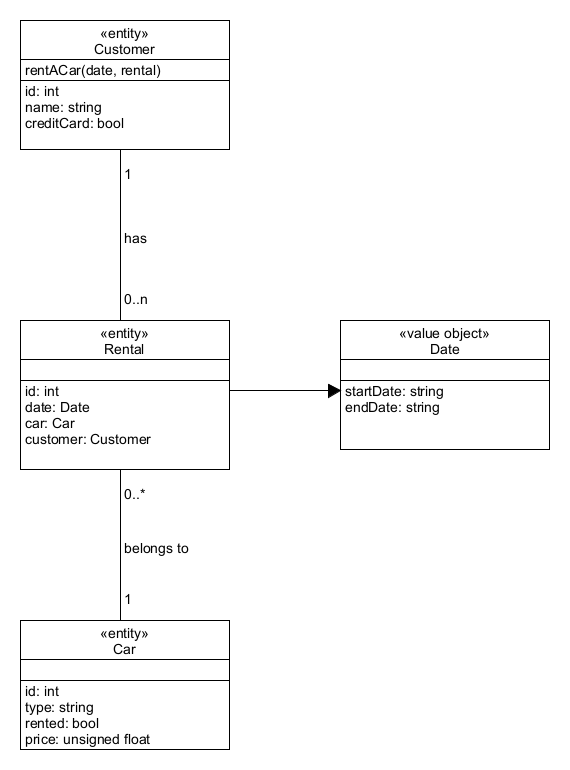
\includegraphics[width=0.6\textwidth]{figures/goLang/carRental/carRental_extendedEntity.png}
    \caption{Extended Entity Diagram}
    \label{fig:extendedEntityDiagram}
\end{figure}

\subsubsection*{Adding the Functionality as a Method}
The chosen signature of the funcion is \texttt{rentACar(startDate: string, endDate: string, rentalId: int, carId: int): Rental}.

The method works as follows:
First, the function checks if the credit card of the customer is valid.
If this is not the case, the function aborts.
Then, the date object is created with the given start and end date.
The algorithm checks if the car is available for the given time period.
If this is not the case, the function aborts.
A new rental object is created with an unique id and is assigned the date object.
The car is marked as rented and linked to the rental object.
The rental object is linked to the customer.
In the end, all changes are saved to the objects and the rental object is returned.

\subsection{Excercise CarRentalExampleData}
\label{sec:exercise_car_rental_example_data}
\subsubsection*{Analyze Alice's Rental Request}
Yes, the request is successful for a number of reasons.

First, the car exists so it can be rented.
Next, the car is not rented for the specified time period.
The only rental of the car is from 1.3.00 to 15.03.2000 by Max.
Finally, Alice is not registered yet, but will be added to the customers table.

Therefore the request is successful and the car is rented to Alice.

\subsubsection*{Add Further Rentals}
This section contains the tables for the customers, cars and rentals as specified in the task sheet.
The task is to add further rentals to the already existing data.
One of the rentals should be a non-conflicting rental, the other one should be conflicting.

The following data is added to the tables:
First, Rental6 is added to the rentals table in \autoref{tab:carRentalExampleDataRentals}.
It is a non-conflicting rental of Car1 by Max from 1.1.05 to 2.2.05.
Next, Rental7 is added to the rentals table.
It is a conflicting rental of Car5 by Bob from 3.1.00 to 10.1.00.
Due to this rental overlapping with Rental5, Rental7 is not a valid rental.

\begin{table}[H]
    \centering
    \caption{Customers Table}
    \label{tab:carRentalExampleDataCustomers}
    \begin{tabular}{|p{2cm}|p{2cm}|}
        \hline
        \multicolumn{2}{|c|}{\textbf{Customers}} \\
        \hline
        \textbf{ID} & \textbf{Name} \\
        \hline
        Cus1 & Max \\
        Cus2 & Bob \\
        Cus3 & Simon \\
        \hline
    \end{tabular}
\end{table}

\begin{table}[H]
    \centering
    \caption{Cars Table}
    \label{tab:carRentalExampleDataCars}
    \begin{tabular}{|p{2cm}|p{3cm}|}
        \hline
        \multicolumn{2}{|c|}{\textbf{Cars}} \\
        \hline
        \textbf{ID} & \textbf{Type} \\
        \hline
        Car1 & VW ID.2 \\
        Car2 & Tesla Model 3 \\
        Car3 & Seat Leon \\
        Car4 & Fiat500e \\
        Car5 & Audi A3 \\
        \hline
    \end{tabular}
\end{table}

\begin{table}[H]
    \centering
    \caption{Rentals Table}    
    \label{tab:carRentalExampleDataRentals}
    \begin{tabular}{|p{2cm}|p{2cm}|p{2cm}|p{2cm}|p{3cm}|}
        \hline
        \multicolumn{5}{|c|}{\textbf{Rentals}} \\
        \hline
        \textbf{ID} & \textbf{StartDate} & \textbf{EndDate} & \textbf{CardID} & \textbf{CustomerID} \\        
        \hline
        Rental1 & 1.3.00 & 15.3.00 & Car1 & Cus1 \\
        Rental2 & 3.2.00 & 5.2.00 & Car2 & Cus2 \\
        Rental3 & 5.1.00 & 1.6.00 & Car3 & Cus2 \\
        Rental4 & 7.2.00 & 25.3.00 & Car4 & Cus3 \\
        Rental5 & 3.1.00 & 5.2.00 & Car5 & Cus3 \\
        Rental6 & 1.1.05 & 2.2.05 & Car1 & Cus1 \\
        Rental7 & 3.1.00 & 10.1.00 & Car5 & Cus2 \\
        \hline
    \end{tabular}
\end{table}

\subsubsection*{Write YAML Code}
The following YAML-code represents the the data from the tables above.
YAML is a human-readable data serialization language, similar to JSON.
The notation specifies an object and the according attributes, storing the data in a key-value format.

\begin{lstlisting}[
    style=kit-cm,
    caption={YAML Code representing the Customers Table},
    label={lst:carRentalExampleDataYaml}
]
- id:   Cus1
  name: Max

- id:   Cus2
  name: Bob

- id:   Cus3
  name: Simon
\end{lstlisting}

\begin{lstlisting}[
    style=kit-cm,
    caption={YAML Code representing the Cars Table},
    label={lst:carRentalExampleDataYamlCars}
]
- id:   Car1
  type: VW ID2

- id:   Car2
  type: Tesla Model 3

- id:   Car3
  type: Seat Leon

- id:   Car4
  type: Fiat 500e

- id:   Car5
  type: Audi A3
\end{lstlisting}

\begin{lstlisting}[
    style=kit-cm,
    caption={YAML Code representing the Rentals Table},
    label={lst:carRentalExampleDataYamlRentals}
]
-   id: Rental1
    startdate:
        day:    1
        month:  3
        year:   2000
    enddate:
        day:    15
        month:  3
        year:   2000
    carid:      Car1
    customerid: Cus1

-   id:         Rental2
    startdate:
        day:    3
        month:  2
        year:   2000
    enddate:
        day:    5
        month:  2
        year:   2000
    carid:      Car2
    customerid: Cus2

-   id:         Rental3
    startdate:
        day:    5
        month:  1
        year:   2000
    enddate:
        day:    1
        month:  6
        year:   2000
    carid:      Car3
    customerid: Cus2

-   id:         Rental4
    startdate:
        day:    7
        month:  2
        year:   2000
    enddate:
        day:    25
        month:  3
        year:   2000
    carid:      Car4
    customerid: Cus3

-   id:         Rental5
    startdate:
        day:    3
        month:  1
        year:   2000
    enddate:
        day:    5
        month:  2
        year:   2000
    carid:      Car5
    customerid: Cus3

-   id:         Rental6
    startdate:
        day:    1
        month:  1
        year:   2005
    enddate:
        day:    1
        month:  1
        year:   2000
    carid:      Car6
    customerid: Cus4

-   id:         Rental7
    startdate:
        day:    3
        month:  1
        year:   2000
    enddate:
        day:    5
        month:  2
        year:   2000
    carid:      Car5
    customerid: Cus4
\end{lstlisting}
